\documentclass[onecolumn,10pt]{article}
\usepackage{geometry}
\geometry{left=10mm,right=10mm,top=30mm,bottom=30mm}
\usepackage{amsmath}
\usepackage{amsthm}
\setlength{\columnsep}{20pt} 
\bibliographystyle{apalike}
\usepackage[labelfont=bf,textfont=bf]{caption}
\setcounter{tocdepth}{2}


\usepackage[dvipdfmx]{graphicx,color}
\graphicspath{ {./figures/} }
\usepackage[dvipdfmx]{hyperref}
\usepackage{pxjahyper}
\hypersetup{% hyperrefオプションリスト
 setpagesize=false,
 bookmarksnumbered=true,%
 bookmarksopen=true,%
 colorlinks=true,%
 linkcolor=blue,
 citecolor=red,
}
\renewcommand\thefootnote{*\arabic{footnote}} %脚注を*1, *2, *3の形に変更

\title{Bayesian Personalized Ranking (BPR) } 
%\author{\href{https://twitter.com/sunbluesome}{ハレハレ (@sunbluesome)}}  
\author{井上 晴幾}
\date{\today}
%%%%%%    TEXT START    %%%%%% 
\begin{document} 
\maketitle 
\tableofcontents
\newpage

\section{Background}
ランキング最適化問題。「アクションのあったものは無かったものより好まれる」という前提のもと、ユーザーに対してrecommendすべきアイテムのランキング問題を解く。recommendの事後確率を最大化するように最適化する。

\section{Fomalization}
$U$は全ユーザー、$I$は全アイテムとし、アクションのあった組み合わせ$S$を
\begin{align}
	S \subseteq U \times I
\end{align}
と定義する。この時、personalized total ranking $>_u \subset I^2$を決定する問題を考える。$>_u$は以下の全順序性(totality, antisymmetry, transitivity)を満たす必要がある。
\begin{align}
	\forall i, j \in I &: i \neq j \Rightarrow i >_u j \lor j >_u i \\
	\forall i, j \in I &: i >_u j \land j >_u i \Rightarrow i = j \\
	\forall i, j \in I &: i >_u j \land j >_u k \Rightarrow i >_u k
\end{align}
また、便宜的に以下を定義する。
\begin{align}
	I_{u}^{+}  &:= \left\{i \in I : (u, i) \in S \right\} \\
	U_{u}^{+}  &:= \left\{u \in U : (u, i) \in S \right\}
\end{align}
以上を元に、データのペアを「アクション有り/無し」で比較する。アクション有りのものは他のものより好まれているとし、以下のようにトレーニングデータセットを作成する。両方ともアクション有り/無しの場合は学習できないのでトレーニングデータからは除外する。
\begin{align}
	D_s := \left\{(u, i, j) | i \in I_{u}^{+} \land j \in I \setminus  I_{u}^{+} \right\}
\end{align}
なお、$D_s$に含まれない欠損値に関しては将来的にはランキングされるべきもの。テストデータとして用いるので$D_s$とテストデータが独立であることが保証される。

\section{Bayesian Personalized Ranking (BPR)}
\subsection{BPR Optimization Criterion}
モデルの事後確率最大化を考える。
\begin{align}
	\mathrm{Max} \;\;\; p(\theta | >_u) \propto p(>_u | \theta)p(\theta)
\end{align}
$\theta$はモデルのパラメータ、$>_u$はユーザー$u$に関する順序構造。全ユーザーを考慮に入れた尤度関数$ p(>_u | \theta)$は以下のように書き直せて
\begin{align}
	\prod_{u \in U} p(>_{u} | \theta) &= \prod_{(u, i, j) \in U \times I \times I} p(i >_u j | \theta)^{\delta((u, i, j) \in D_s)} \cdot \left( 1 -   p(i >_u j | \theta)^{\delta((u, i, j) \not\in D_s)} \right)
\end{align}
\begin{equation}
\delta (b) = \left\{
\begin{array}{ll}
1 & \mathrm{if}\;b\; \mathrm{is\;true} \\
0 & \mathrm{else}
\end{array}
\right.
\end{equation}
完全性と反対称律から
\begin{align}
	\prod_{u \in U} p(>_{u} | \theta) = \prod_{(u, i, j) \in D_s} p(i >_u j | \theta)
\end{align}
と書ける。また、
\begin{align}
	p(i >_u j | \theta) :=& \sigma \left(\hat x_{uij} \left(\theta \right) \right) \\
	\sigma \left( x \right) :=& \frac{1}{1 + e^{-x}}
\end{align}
と定義する。$\hat x_{uij} \left( \theta \right)$の推定をMFやkNNに投げる。この枠組みなら$D_s$についてのみ尤度が計算されるので、「0」を学習することによる過学習も起きない。

\subsection{BPR-OPTの導出}
事前分布は以下のように設定する。
\begin{align}
	p(\theta) &\sim \mathcal{N}\left(0, \Sigma_{\theta} \right) \\
	\Sigma_{\theta} = \lambda_{\theta} I &\Rightarrow \Sigma^{-1}_{\theta} = \frac{1}{\lambda_{\theta}} I
\end{align}
この時、対数尤度関数BPR-OPTを以下のように定義する。
\begin{align}
	\mathrm{BPR-OPT} &:= \ln p\left(\theta | >_u \right) \\
	&\propto \ln p\left(>_u | \theta \right) p(\theta) \\
	&= \ln \prod_{(u,i,j) \in D_s} \sigma \left( \hat x_{uij} \left(\theta \right) \right) p \left(\theta \right) \\
	&= \Sigma_{(u,i,j) \in D_s} \ln \sigma \left( \hat x_{uij} \left(\theta \right) \right) + \ln p \left(\theta \right) \\
	&\propto  \Sigma_{(u,i,j) \in D_s}  \ln \sigma \left( \hat x_{uij} \left(\theta \right) \right) - \frac{1}{2\lambda_\theta} \|\theta\|
\end{align}

\subsection{Analogies to AUC optimization}
ユーザーごとの$AUC$を以下のように定義する。
\begin{align}
	AUC(u) := \frac{1}{| I_u^+ || I \setminus I_u^+ |} \Sigma_{i \in I_u^+}\Sigma_{j \in I \setminus I_u^+} \delta (\hat x_{uij} > 0)
\end{align}
これより、$AUC$の平均は
\begin{align}
	AUC_{ave} &:= \frac{1}{|U|} \Sigma_{u \in U} AUC(u) \\
	&= \Sigma_{(u,i,j) \in D_s} z_u \delta (\hat x_{uij} > 0) \\
	z_u &= \frac{1}{|U| | I_u^+ | |I \setminus I_u^+ |} \\
	\delta (x > 0) &= H(x) = 1\;\mathrm{if}\; x>0, \; \mathrm{else}\; 0
\end{align}
$H(x)$はヘヴィサイド関数(step関数)の意味。微分不可能なのでsigmoid関数でよく置き換えられる。

\subsection{BPR Learning Algorithm}
対数尤度関数BPR-OPTの極値を求める。
\begin{align}
	\frac{\partial \mathrm{BPR\mathchar`-OPT}}{\partial \theta} &= \Sigma_{(u,i,j) \in D_s} \frac{\partial}{\partial \theta} \ln \sigma \left(\hat x_{uij} (\theta ) \right) - \frac{1}{2\lambda_{\theta}}\frac{\partial}{\partial \theta}\|\theta\|^2 \\
	&= \Sigma_{(u,i,j) \in D_s} \left(1+e^{- \hat x_{uij}(\theta)} \right)\left(1+e^{- \hat x_{uij}(\theta)} \right)^{-2} \cdot \left(-e^{- \hat x_{uij}(\theta)} \right) \frac{\partial}{\partial \theta} \hat x_{uij} - \frac{1}{\lambda_{\theta}} \theta \\
	&\propto \Sigma_{(u,i,j) \in D_s} \frac{-e^{- \hat x_{uij}(\theta)}}{1+e^{- \hat x_{uij}(\theta)}}\frac{\partial}{\partial \theta} \hat x_{uij} \left(\theta \right) - \frac{1}{\lambda_{\theta}}\theta
\end{align}
これを用いてSGDを行い、BPR-OPTの極値を求める。

\subsection{Learning models with BPR}
MFとkNNはuser-itemペア$(u,l)$に対して実数$\hat x_{ul}$を求める問題。$(u,i,j) \in D_s$は3要素なので$\hat x_{uij}$を以下のように分解・定義する。
\begin{align}
	\hat x_{uij} := \hat x_{ui} - \hat x_{uj}
\end{align}
$\hat x_{ul}$だけを回帰しようとする他の方法と異なり、$\hat x_{ui} - \hat x_{uj}$を分類する問題(triplet loss)となっている。アルゴリズムは論文参照(ただのSGDだけど)。

\subsection{Matrix Factorization}
以下のような$X: U \times I$を推定する問題(Fig. \ref{fig:MF_1})。
\begin{align}
	\hat X &:= WH^T \\
	W &: |U| \times k, H: |I| \times k \\
	k &: dimensinality / rank
\end{align}
\begin{figure}[htbp]
	\centering
	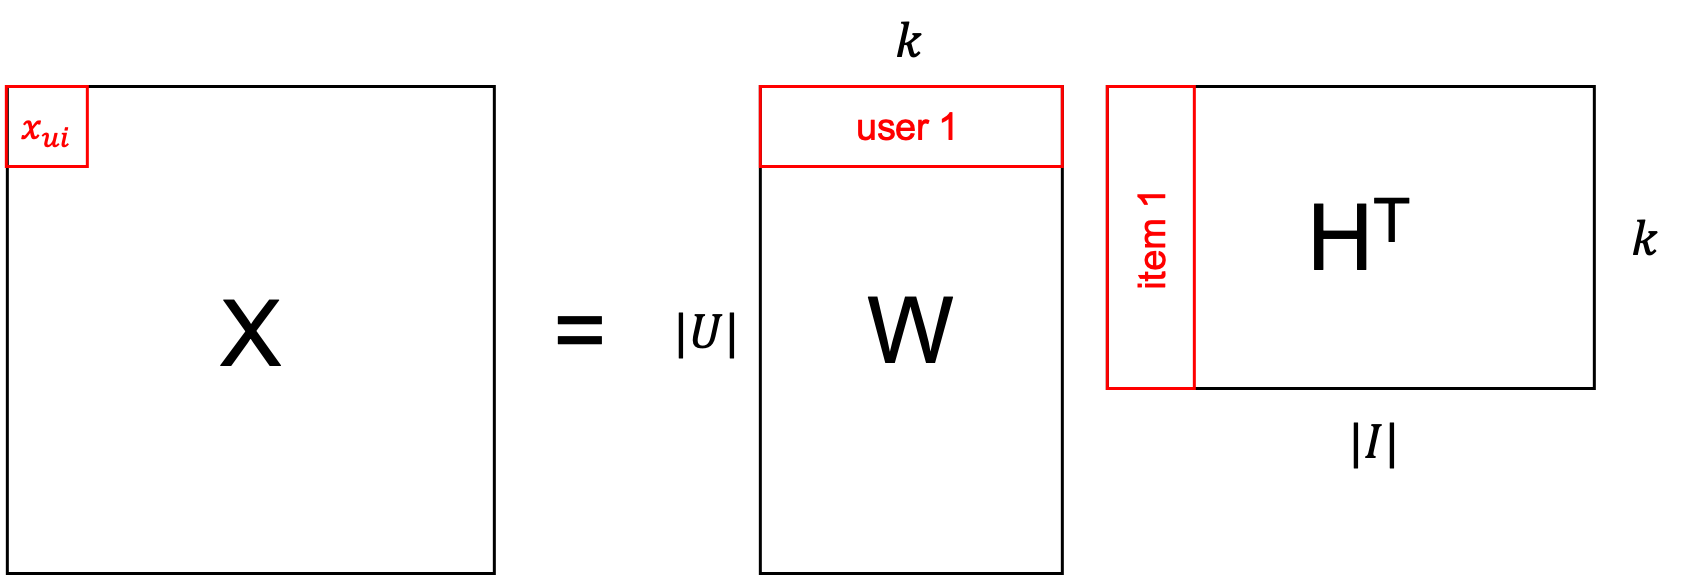
\includegraphics[width=0.5\linewidth]{MF.png}
	\caption{Matrix Factorization}
	\label{fig:MF_1}
\end{figure}

また、予測式は以下のように書き直せる。
\begin{align}
	\hat x_{ui} &= \left<w_u, h_i \right> = \Sigma_{f=1}^{k} w_{uf}h_{if} \\
	\theta &= \left(W, H \right)
\end{align}
$\hat x_{ui}$にはlinear kernel$ \left<w_u, h_i \right>$を用いたが、他のカーネルも使える(RBFカーネルなど)。BPRはgradient descentを使っているので$\partial \hat x_{uij} / \partial \theta$を計算しておく必要がある。

\begin{align}
	\hat x_{uij} = \hat x_{ui} - \hat x_{uj} = \left<w_u, h_i \right> - \left<w_u, h_j \right>
\end{align}
より、
\begin{equation}
	\frac{\partial \hat x_{uij}}{\partial \theta} = \left\{
		\begin{array}{ll}
			h_{if} - h_{jf} & \mathrm{if}\;\theta = w_{uf} \\
			w_u & \mathrm{if}\;\theta = h_{if} \\
			-w_u & \mathrm{if}\;\theta = h_{jf} \\
			0 & \mathrm{else}
		\end{array}
	\right.
\end{equation}
これを、SGDの更新式
\begin{equation}
	\theta \leftarrow \theta + \alpha \left( \Sigma_{(u,i,j) \in D_s} \frac{e^{- \hat x_{uij}(\theta)}}{1+e^{- \hat x_{uij}(\theta)}}\frac{\partial}{\partial \theta} \hat x_{uij} \left(\theta \right) + \frac{1}{\lambda_{\theta}}\theta \right)
\end{equation}
で用いる。$\lambda_\theta$は更新するパラメータごとに設定される(MFでは合計3つ)

\subsection{Adaptive k-Nearest Neighbor}
\begin{enumerate}
	\item item-based と user-basedの2通りがある
	\item 類似度の選び方に依存する
\end{enumerate}

ユーザーにが過去に見た全アイテムと、特定のアイテム$i$との類似度を以下のように計算する。
\begin{align}
	\hat x_{ui} = \Sigma_{l \in I_{u}^{+} \land l \neq i} c_{il}, \;\;\; c \in C,  C: I \times I 
\end{align}
ここで、$C$の計算はヒューリスティックに行われ、例えば
\begin{align}
	c_{ij}^{cosine} := \frac{|U_{i}^{+} \cap U_{j}^{+} |}{\sqrt{|U_{i}^{+}||U_{j}^{+}|}}
\end{align}
である。「metric learningしてしまった方が良い」と論文では述べている。$HH^T$のようにMFしてしまうという手もある。以上より、
\begin{align}
	\hat x_{uij} = \hat x_{ui} - \hat x_{uj} = \Sigma_{l \in I_{u}^{+} \land l \neq i}  c_{il} - \Sigma_{l \in I_{u}^{+} \land l \neq j}  c_{jl} \\
	\frac{\partial \hat x_{uij}}{\partial \theta} = \left\{
		\begin{array}{ll}
			+1 & \mathrm{if}\;\theta \in \left\{c_{il}, c_{li} \right\} \land l \in I_{u}^{+} \land l \neq i  \\
			-1 & \mathrm{if}\;\theta = \in \left\{c_{jl}, c_{lj} \right\} \land l \in I_{u}^{+} \land l \neq j \\
			0 & \mathrm{else}
		\end{array}
	\right.
\end{align}
このときの正則化パラメータ$\lambda_\theta$は2つである。

\end{document}